% TIPOLOGIA DI DOCUMENTO
\documentclass{report}

% PACCHETTI INSERITI 
\usepackage{graphicx} % Per le immagini
\usepackage{amsmath} % Simboli matematici
\usepackage[hidelinks]{hyperref} % Collegamenti ipertestuali
\usepackage{amssymb} % Simboli matematici 2
\usepackage{array}
\usepackage[table]{xcolor}
\usepackage{multicol}
\usepackage{fancyvrb}
\usepackage{cancel}
\usepackage{geometry}
\usepackage{listings}
\usepackage{xcolor}
\usepackage{soul}
\usepackage{listings}
\usepackage{algorithm}
\usepackage{mathabx}
\usepackage{algpseudocode}
\usepackage{mathrsfs}

\definecolor{purp}{rgb}{0.875, 0.702, 0.961}
\newcommand{\mathcolorbox}[2]{\colorbox{#1}{$\displaystyle #2$}}

\renewcommand{\thelstnumber}{\arabic{lstnumber}:}
\lstdefinestyle{mystyle}{          
	numbers=left,                    
	numbersep=5pt             
}
\lstset{style=mystyle}

\geometry{
	a4paper,
	total={160mm,260mm},
	left=30mm,
	top=18mm,
}


% RIDENOMINAZIONI
\renewcommand{\chaptername}{Capitolo}
\renewcommand{\contentsname}{Indice}
\renewcommand{\figurename}{Immagine}
\renewcommand{\tablename}{Tabella}
\makeatletter
\renewcommand{\ALG@name}{Algoritmo}
 \makeatother
\setcounter{chapter}{-1}

% TITOLO, INDICE
\title{\Huge\textbf{Computabilità e Complessità}}
\author{Damiano Trovato}
\date{Secondo semestre, anno 2025/26}

\begin{document}
	\maketitle
	\newpage
	\tableofcontents
	\newpage
	
	\chapter{Introduzione alla computabilità}
	
	\section{I personaggi della computabilità}
	
	\paragraph{Gottfried Wilhelm Von Leibniz} Tra gli inizi del 600 e la fine del 700: un grande ottimismo, che pensava il mondo fosse stato sviluppato nel modo migliore. In un epoca senza computer e tecnologia tale per svilupparli, definisce un linguaggio chiamato \textbf{Caratteristica Universale}. Si pongono le basi per la \textbf{logica del primo ordine}, il \textbf{calcolo deduttivo}. Ogni disputa si sarebbe dovuta risolvere con un calcolo! Ricordiamo il contributo di Leibniz all'analisi matematica con il concetto di \textbf{derivata} e la notazione che usiamo oggi: queste notazioni ammettevano delle automazioni! Contribui anche alla creazione di un meccanismo, noto come \textbf{ruota di Leibniz}, che estendeva l'addizionatrice di Pascal con le moltiplicazioni. Di fronte al tentativo di ricavare l'assioma delle parallele, si inizia a definire il concetto di \textbf{consistenza delle teorie}. In generale, fu il primo a mettere le basi per un \textbf{calcolo universale}. 
	
	\paragraph{George Boole} Algebrizza la logica proposizionale, ridefinendo il ragionamento usando connettivi logici ($\land, \lor, \lnot$).
	
	\paragraph{Gottlob Frege} Definito spesso come il padre della logica matematica formale. La logica di Frege usava anche molti elementi di teoria degli insiemi.
	
	\paragraph{William Russell} Uno dei paradossi posti a Frege, e probabilmente uno dei paradossi più grandi della storia della logica.
	Sia $U$ l'insieme di tutti gli insiemi che non contengono se stessi. $U$ appartiene a se stesso?
	$$
	U = \{x : x \notin x\}; \qquad U \in U ?
	$$
	
	Questo mette in crisi un'assioma della logica di Frege, noto come \textbf{assioma di appartenenza}, fin troppo potente, tale da causare il paradosso 
	
	$$
	U \in U \implies U \notin U, \quad U \notin U \impliedby U \in U, \quad U \in U \Leftrightarrow U \notin U
	$$
	
	\paragraph{Georg Cantor} Definisce la tecnica di \textbf{diagonalizzazione}: data una lista infinita, è possibile creare un elemento che non appartiene a questa lista, utile per alcune dimostrazioni.
	
	\paragraph{David Hilbert} Vanno definite le regole in maniera chiara e univoca, per creare un formalismo di logica e deduzione veramente consistente e rigoroso. La matematica è una scienza che deve consentire un modo per dimostrare in maniera esatta i propri statement: devono quindi essere definiti, dalla comunità, assiomi e regole di deduzione di ciascun sistema. Vengono quindi definiti i problemi di Hilbert, una celebre lista di 23 quesiti matematici. Non tra questi, è il problema della decidibilità.
	
	\paragraph{Kurt Gödel} Dimostra il \textbf{teorema di incompletezza}, secondo qui non è possibile dimostrare la consistenza della matematica con i metodi dell'artimetica (come David Hilbert sperava): alcune cose vanno date per buone! Meno cose possibili, ma qualcosa sì. Le dimostrazioni di consistenza dell'aritmetica utilizzano elementi di teoria degli ordinali\footnote{La teoria degli ordinali, sviluppata da Cantor, generalizza il concetto di posizione (primo, secondo...) agli insiemi infiniti, andando oltre i numeri naturali. Un numero ordinale è un insieme ben ordinato, dove ogni ordinale è l'insieme di tutti gli ordinali precedenti}. Il concetto di verità non può essere definito con metodi finiti. L'aritmetica non può dimostrare tutte le asserzioni: queste possono comunque essere vere!
	
	\paragraph{Alonzo Church} Dimostra che l'artimetica è indecidibile, introducendo un calcolo formale noto come $\lambda$-calcolo.
	
	\paragraph{Alan Turing} Un contemporaneo di Alonzo Church, formalizza la prima \textbf{macchina teorica universale}, nota come \textbf{Macchina di Turing}. Da lì nasce l'idea di creare un calcolatore capace di simulare tutte le altre macchine. Nasce l'\textbf{Halting Problem}, che si dimostra non risolvibile con il metodo di diagonalizzazione.
	
	\section{Cos'è un algoritmo?}
	Nonostante moltissimi algoritmi siano stati applicati negli anni per risolvere problemi tipici (le 4 operazioni, problema di Euclide, crivello di Eratostene, fattorizzazione o test di divisibilità), per molto tempo \textbf{non è stato definito il concetto di algoritmo}. Un algoritmo è una procedura descritta in maniera univoca usando un formalismo opportuno. Può anche essere linguaggio naturale, ma \textbf{nulla deve essere definito in maniera ambigua} (niente \textit{"sale q.b."}).
	
	\subsection{Risolvere un algoritmo}
	
	\paragraph{Risolvere in positivo un algoritmo}
	Significa dimostrare l'esistenza di un algoritmo. Questa coincide con l'algoritmo stesso. È sufficiente esibire l'algoritmo stesso in un formalismo coerente e univoco.
	
	\paragraph{Risolvere in negativo un algoritmo}
	Significa dimostrare che tra tutti gli algoritmi possibili, nessuno risolve il problema posto.
	La dimostrazione di non-esistenza di algoritmo deve essere necessariamente accompagnata da una definizione univoca di algoritmo tramite un opportuno \textbf{sistema di calcolo universale}. 
	
	\subsection{Congettura di Church-Turing}
	Si dimostra che esiste un'equivalenza tra i vari sistemi formali definiti fino ad ora. La congettura di Church-Turing afferma che ogni sistema formale si rifà a quelli già noti. Si osserva che questa congettura può essere solo confutata, ma non dimostrata.
	
	\newpage
	
	\chapter{Funzioni computabili e URM}
	
	Apriamo il corso definendo l'idea di algoritmo, mostrando come questo possa essere descritto in maniera precisa usando un computer ideale (Macchina a Registri Illimitati), ponendo le basi per la teoria della computabilità.
	
	\section{Unlimited Register Machine}
	Una \textbf{Unlimited Register Machine} è una macchina teorica costituita da un array \textit{potenzialmente} infinito, costituito da registri $R_1, R_2, \dots$ ciascuno dei quali può contenere un numero naturale a precisione infinita. L'informazione non è infinita, in quanto tutti i registri contengono il valore zero, a meno dei registri usati, i quali sono in un numero finito.
	Lo stato di una URM è contenuto nei suoi registri $\vec{r} \in \mathbb{N}^\infty$. Un algoritmo che cambia lo stato interno della URM è detto \textbf{URM-programma}. 
	Un URM-programma è una sequenza finita di $s$ istruzioni $I_1, I_2, \dots, I_s$. 
	\subsection{Configurazione istantanea}
	È una coppia del tipo $(k, \vec{r}) \in \mathbb{N}^+\times \mathbb{N}^\infty$, dove $k$ si chiama  \textbf{contatore di programma}, e rappresenta l'indice dell'istruzione $I_k$ che sta per essere eseguita, mentre $\vec{r}$ è lo stato. 
	
	
\begin{figure}[tbph]
	\centering
	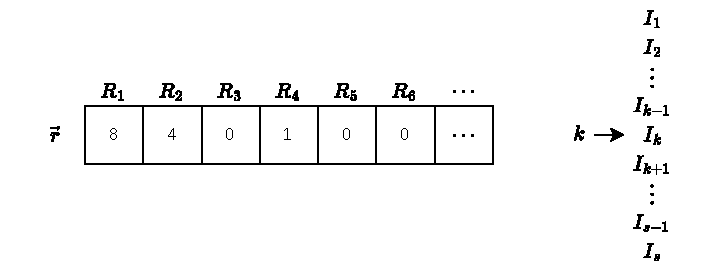
\includegraphics[width=0.7\linewidth]{images/configurazione}
\end{figure}

La configurazione istantanea corrente è $(k, (8,4,0,1,0,0,\dots))$.
	
	\subsection{Istruzioni degli URM-programmi}
	\emph{Un URM-programma è una sequenza finita di $s$ istruzioni $I_1, I_2, \dots, I_s$}. Tra queste, abbiamo:
	\begin{multicols}{2}
	\begin{itemize}
		\item Reset
		\item Incremento
		\item Assegnamento (non necessaria)
		\item Salto condizionato
	\end{itemize}
	\end{multicols}
	
	\paragraph{Istruzione di Reset} $Z(n)$. Azzera il valore contenuto dello slot $n$-esimo. 
	
	$$
	(k, \vec{r}) \xrightarrow{Z(n)} (k+1, \vec{r'}) \quad r_i' = \begin{cases}
	r_i, i \neq n\\
	0, i = n
	\end{cases}
	$$
	
	\paragraph{Istruzione di Incremento} $S(n)$. Incrementa di 1 il valore contenuto dello slot $n$-esimo. 
	
	$$
	(k, \vec{r}) \xrightarrow{S(n)} (k+1, \vec{r'}) \quad r_i' = \begin{cases}
	r_i, i \neq n\\
	r_i +1, i = n \end{cases}
	$$
	
	\paragraph{Istruzione di Assegnamento} $T(m,n)$. Assegna allo slot $n$-esimo il valore contenuto nello slot $m$-esimo. 
	
	$$
	(k, \vec{r}) \xrightarrow{T(m, n)} (k+1, \vec{r'}) \quad r_i' = \begin{cases}
		r_i, i \neq n\\
		r_m, i = n \end{cases}
	$$
	
	\paragraph{Istruzione di Salto condizionato} $J(m,n, q)$. Lo stato rimane lo stesso, ma cambia il contatore di programma $k$.
	
	$$
	(k, \vec{r}) \xrightarrow{J(m, n, q)} (k', \vec{r}) \quad k' = \begin{cases}
		k+1, m \neq n\\
		q, m = n \end{cases}
	$$
	
	
	\section{Definizione di computazione}
	
	Sia $P = \{I_1, I_2, \dots, I_s\}$ un \textbf{programma} con $s$ istruzioni, e $\vec{r}$ lo stato dei registri. La computazione $P(\vec{r})$ di $P$ a partire dallo stato $\vec{r}$ è la sequenza (finita o infinita) di configurazioni istantanee con $k_1 = 1, \vec{r}^{(1)}=\vec{r}$.
	$$
	(k_1, \vec{r}^{(1)}),\;
	(k_2, \vec{r}^{(2)}),\;
	(k_3, \vec{r}^{(3)}),\;
	\ldots,\;
	(k_z, \vec{r}^{(z)}),\;
	(k_{z+1}, \vec{r}^{(z+1)}),\;
	\ldots
	$$
	
	tra queste configurazioni, identifichiamo
	
	\begin{itemize}
		\item Configurazione iniziale, $(1, \vec{r})$.
		\item Configurazione $i$-esima con successore, $(k_i, \vec{r}^{(i)})$. Se $k_i \leq s$, allora ha un successore nella computazione $P(\vec{r})$, e si ha $(k_i, \vec{r}^{(i)}) \xrightarrow{I_{k_{i+1}}} (k_i, \vec{r}^{(i+1)})$
		\item Configurazione finale, $(k_i, \vec{r}^{(i)})$. Se $k_i > s$, allora non ha un successore nella computazione $P(\vec{r})$, e quindi è la \textbf{configurazione finale} della stessa. Si arriva alla configurazione finale tramite esecuzione lineare o salti condizionali.
	\end{itemize}
	
	introduciamo quindi una notazione: $P(\vec{r})$ è un programma con stato iniziale $\vec{r}$,
	$$
	r_i =
	\begin{cases}
		a_i & \text{se } i <n \\
		0 & \text{altrimenti}
	\end{cases}
	$$
	
	$$
	P(a_1, a_2, \ldots, a_n)
	\equiv
	P(a_1, a_2, \ldots, a_n, 0, 0, \ldots)
	$$
	
	In particolare, possiamo indicare se la computazione termina o meno.
	\begin{itemize}
		\item $P(\vec{r})\downarrow$ è una computazione \textbf{terminante};
		\item $P(\vec{r})\uparrow$ è una computazione \textbf{non terminante}
	\end{itemize}
	
	Solitamente, il registro $R_1$ viene usato per l'input e l'output della computazione. Nella notazione, scriveremo che la computazione che torna $b$, $P(\vec{r})\downarrow b$. 
	
	
	\section{Funzione parziale}
	Definiamo $f: A \to B$ funzione parziale, tale che $\text{Dom}(f) \subseteq A$, per cui il dominio potrebbe non essere tutto $A$. Per $a \in A$, se $f$ è definita su $a$, $f(a)\downarrow$, altrimenti $f(a)\uparrow$.
	
	Se $f,g : A \to B$ funzioni parziali, diremo che $f \simeq g$ se:
	\begin{enumerate}
		\item $\forall a \in A: \ f(a)\downarrow \Leftrightarrow g(a)\downarrow$
		\item $\forall a \in A: \ f(a)\downarrow \implies f(a) = g(a) $
	\end{enumerate}
	
	con questa notazione che riprende la terminazione (o non terminazione) dei programmi URM, possiamo indicare se una funzione è definita per un determinato valore dell'insieme $A$.
	
	
	\subsection{Funzioni URM-calcolabili}
	Sia $P$ un programma. $\forall n \geq 1$, poniamo
	$$
	f_P^{(n)}(a_1, a_2, \ldots, a_n) =
	\begin{cases}
		b & \text{se } P(a_1, a_2, \ldots, a_n) \downarrow b \\[6pt]
		\uparrow & \text{se } P(a_1, a_2, \ldots, a_n) \uparrow
	\end{cases}
	$$
	
	chiameremo la funzione parziale $f_P^{(n)} : \mathbb{N}^n \to \mathbb{N}$ la funzione $n$-aria calcolata dal programma $P$.
	Una funzione parziale $g$ si dirà \textbf{URM-calcolabile} se esiste un programma URM $P$ tale che $g \simeq f_P^{(n)}$.

	\paragraph{L'insieme $\mathcal{C}^\text{URM}$ e $\mathcal{C}_n^\text{URM}$}
	La collezione di tutte le funzioni URM-calcolabili  di qualunque arietà si indica con $\mathcal C^\text{URM}$. La collezione di tutte le funzioni URM calcolabili $n$-arie si indica con $\mathcal C_n^\text{URM}$. Scopriremo poi, con la congettura di Church-Turing, che $\mathcal C^\text{URM} = \mathcal C$.
	
	\paragraph{$\mathcal{C}$ è enumerabile} Dimostriamo ciò osservando che $\mathcal{C} = \bigcup_{n=1}^\infty \mathcal C_n^\text{URM}$, e che ciascuna delle $\mathcal C_n$ è costituita da istruzioni del tipo $S(n), Z(n), T(m,n), J(m,n,q)$, che sono enumerabili. Questo vuol dire che il dominio di $\mathcal C^\text{URM}$ è enumerabile, meno denso dell'insieme di tutte le funzioni $f$. 
	
	\section{Esercizi}
	Si allega interprete di programmi-URM online col quale verificare le proprie soluzioni: \url{https://sites.oxy.edu/rnaimi/home/URMsim.htm}
	\subsection{Programmi URM}
	Si dimostri che le seguenti funzioni sono calcolabili esibendo opportuni programmi URM.
	
\subsubsection{Funzione segno}
$$
f(x) = \begin{cases}
	0 & \text{se } x=0\\
	1 & \text{se } x\neq 0
\end{cases}
$$

\begin{algorithm}[H]
	\caption{Funzione segno}
	\begin{algorithmic}[1]
		\State $J(1,2,4)$
		\State $S(2)$
		\State $T(2,1)$
	\end{algorithmic}
\end{algorithm}

\subsubsection{Funzione costante}
$$
f(x) = 5
$$

\begin{algorithm}[H]
	\caption{Funzione costante}
	\begin{algorithmic}[1]
		\State $Z(1)$
		\State $S(1)$
		\State $S(1)$
		\State $S(1)$
		\State $S(1)$
		\State $S(1)$
	\end{algorithmic}
\end{algorithm}

\subsubsection{Funzione uguaglianza}
$$
f(x, y) = \begin{cases}
	0 & \text{se } x=y\\
	1 & \text{se } x\neq y
\end{cases}
$$

\begin{algorithm}[H]
	\caption{Funzione uguaglianza}
	\begin{algorithmic}[1]
		\State $T(1,3)$
		\State $J(2,3,5)$
		\State $Z(1)$
		\State $S(1)$
	\end{algorithmic}
\end{algorithm}

\subsubsection{Funzione minore o uguale}
$$
f(x, y) = \begin{cases}
	0 & \text{se } x\leq y\\
	1 & \text{se } x> y
\end{cases}
$$

\begin{algorithm}[H]
	\caption{Funzione minore o uguale}
	\begin{algorithmic}[1]
		\State $T(1,3)$
		\State $Z(1)$
		\State $S(2)$
		\State $S(4)$
		\State $J(2,4,8)$
		\State $J(3,4,9)$
		\State $J(1,1,4)$
		\State $S(1)$
	\end{algorithmic}
\end{algorithm}

\subsubsection{Funzione x/3}
$$
f(x) =
\begin{cases}
	\dfrac{1}{3}x & \text{se } x \text{ è un multiplo di } 3 \\[6pt]
	\uparrow & \text{altrimenti}
\end{cases}
$$

\begin{algorithm}[H]
	\caption{Funzione $x/3$}
	\begin{algorithmic}[1]
		\State $T(1,4)$
		\State $Z(1)$
		\State $S(1)$
		\State $S(5)$
		\State $S(5)$
		\State $S(5)$
		\State $J(4,5,9)$
		\State $J(1,1,3)$
	\end{algorithmic}
\end{algorithm}

\subsubsection{Funzione $\lfloor 2x/3 \rfloor$}
$$
f(x) =
\begin{cases}
	\lfloor\dfrac{2}{3}x\rfloor & \text{se } x \text{ è un multiplo di } 3 \\[6pt]
	\uparrow & \text{altrimenti}
\end{cases}
$$

\begin{algorithm}[H]
	\caption{Funzione $\lfloor 2x/3 \rfloor$}
	\begin{algorithmic}[1]
	\State TODO
	\end{algorithmic}
\end{algorithm}
	\subsection{Dimostrazioni}
	
	\subsubsection{L'istruzione $T$ non è necessaria}
	
	\begin{algorithm}[H]
		\caption{Istruzione $T$}
		\begin{algorithmic}[1]
			\State Z(m)
			\State S(m)
			\State J(m,n,1)
		\end{algorithmic}
	\end{algorithm}
	
	\subsubsection{Programma senza istruzioni $J$}
	Sia $P$ un programma URM che non contiene alcuna istruzione del tipo $J(m,n,p)$, si dimostra che esiste $m \in \mathbb{N}$ tale che:
	
	
	\section{Correttezza dei programmi}
	
	\paragraph{Correttezza parziale} Un programma $P$ si dice \textbf{parzialmente corretto} rispetto a date specifiche di input $\alpha$ e di output $\beta$ (note rispettivamente come \textbf{precondizione} e \textbf{postcondizione}) se, per ogni input $\vec{x}$ soddisfacente le specifiche $\alpha$, se l'esecuzione di $P$ su $\vec{x}$ è terminante, allora l'output di $P$ soddisfa le specifiche $\beta$.

	$$
	(\forall \vec{x})(\forall b) [(\alpha(\vec{x}) \land P(\vec{x})\downarrow b) \rightarrow \beta(\vec{x}, b)]
	$$
	
	\paragraph{Correttezza totale} Un programma $P$ si dice totalmente corretto rispetto alle specifiche $\alpha$ e $\beta$ se è parzialmente corretto e vale anche la condizione di terminazione:
	
	$$
	(\forall \vec{x})(\alpha(\vec{x}) \rightarrow P(\vec{x})\downarrow)
	$$
	
	\subsection{Esempio di specifiche}
	\paragraph{Correttezza parziale su funzione sottrazione} $\lambda xy.x-y$. Precondizione: $\alpha(x,y) \equiv x \geq 0 \land y \geq 0$. Postcondizione $\beta(x,y,z) \equiv z = x-y$.
	\paragraph{Correttezza totale su funzione sottrazione} $\lambda xy.x-y$. Precondizione: $\alpha(x,y) \equiv x \geq y \land y \geq 0$. Postcondizione $\beta(x,y,z) \equiv z = x-y$
	
	\subsection{Verifica della correttezza parziale dei programmi di Floyd/Hoare}
	Introduciamo adesso delle metodologie per trovare un'asserzione per cui le condizioni di verifica del programma risultino corrette. Usiamo il seguente programma come esempio:
	$$
	\lambda r_1r_2.(r_1+r_2 )
	$$
	\begin{lstlisting}
J(3,2,5)
S(1)
S(3)
J(1,1,1)
	\end{lstlisting}
	
	\begin{figure}[tbph]
		\centering
		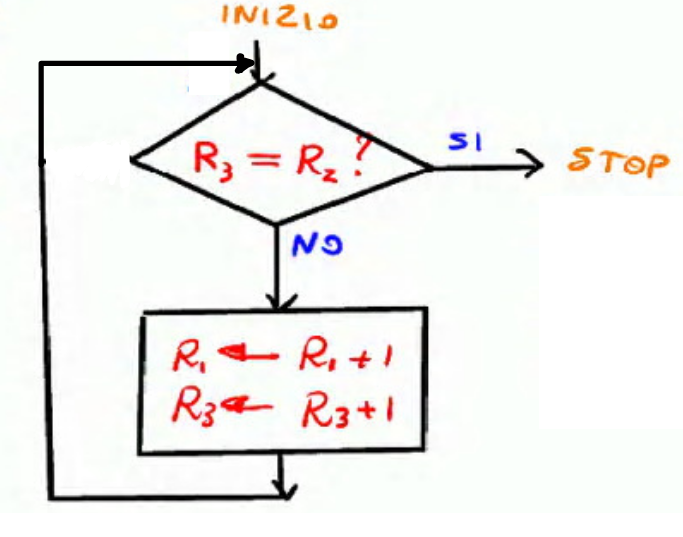
\includegraphics[width=0.5\linewidth]{images/verifica-programma}
	\end{figure}
	
	$$
	precondizione : \begin{cases}
	r_1 = \overline{r_1}\\
	r_2 = \overline{r_2}\\
	r_3 = 0
	\end{cases}
	$$
	
	
	
	\subsection{Verifica della correttezza totale dei programmi}
	Se la verifica della correttezza parziale sfrutta la logica, per la correttezza totale si vuole uno strumento che \textbf{verifica la terminazione} in ogni caso. 
	
	È sufficiente trovare una misura a valori in un insieme ben fondato che decresca strettamente ad ogni iterazione. Possiamo quindi rafforzare l'invariante $A$ con la condizione di decrescita, ottenendo $A^*$. 
	
	\subsection{Sulla verifica della correttezza}
	In generale, metteremo un'asserzione per ogni ciclo condizionale. Il numero di condizioni, invece, è uguale al numero di percorsi.
	
	\section{Predicati}
	Un predicato $n$-ario è una funzione $M : N \to \{true, false\}$. I predicati sono trattati come funzioni, associando ad essi la loro \textbf{funzione caratteristica}.
	
	$$
	c_m(\vec{x}):= \begin{cases}
	1 & \text{se }M(\vec{x})= true\\
	0 & \text{se }M(\vec{x})= false\\
	\end{cases}
	$$
	
	La funzione caratteristica del predicato $x = 0$, ad esempio, è data da
	
	$$
	g(x) = \begin{cases}
	1 & \text{se } x = 0\\
	0 & \text{altrimenti}
	\end{cases}
	$$
	
	\subsection{Predicati decidibili}
	Un predicato si dice \textbf{decidibile} se la sua funzione caratteristica è \textbf{calcolabile}. Scrivere un programma $P$ che calcola la funzione caratteristica è sufficiente per dimostrare che il predicato sia decidibile.
	
	\section{Calcolabilità su altri domini}
	È possibile generalizzare i concetti di decidibilità e calcolabilità ai predicati $M: D \to \{true, false\}$ e funzioni $f : D \to D$ per domini $D \neq \mathbb{N}$: deve esistere tuttavia un modo effettivo per mappare il dominio di $D$ su $\mathbb{N}$.
	
	$$\mathbb{N} \xrightarrow{\alpha^{-1}} D \xrightarrow{f} D \xrightarrow{\alpha} \mathbb{N}$$
	
	Si richiede una codifica effettiva di $D: \alpha: D \to \mathbb{N}$ che sia
	\begin{itemize}
		\item Iniettiva;
		\item Suriettiva;
		\item Effettivamente\footnote{Per effettivo, intendiamo che deve esistere un modo di calcolare la mappatura e l'inversione, un algoritmo vero e proprio.} calcolabile e invertibile.
	\end{itemize}
	
	Definiamo quindi una funzione $f^* = \alpha (f(\alpha^{-1}(x)))$. Questa funzione è calcolabile.
	Un esempio di codifica effettiva per lavorare in $\mathbb{Z}$ è
	
	$$
	\alpha(x) = \begin{cases}
	2x & \text{se } x \geq 0\\
	-2x -1 & \text{altrimenti}
	\end{cases},
	\qquad
	\alpha^{-1}(y) = \begin{cases}
		\dfrac{1}{2}y & \text{se } y \text{ è pari}\\
		-\dfrac{1}{2}(y+1) & \text{altrimenti}
	\end{cases}
	$$
	
	
	
	\chapter{Creare funzioni computabili}
	Tratteremo adesso una serie di metodi per combinare funzioni computabili, ottenendo altre funzioni computabili. Questo ci consentirà di dimostrare che moltissime funzioni sono computabili, senza dover scrivere un programma $P$ ogni volta, renendo meno tedioso il processo di dimostrazione della computabilità.  Prima di definire gli strumenti usati, dobbiamo dimostrare che questi sono validi.
	
	\section{Condizioni di esistenza di programmi}
	Definiremo degli strumenti per capire se una funzione è calcolabile \textbf{senza dover scrivere il programma} che la calcola.
	
	\paragraph{Insieme delle funzioni di base} È un insieme di funzioni  notoriamente calcolabili.
	\begin{itemize}
		\item Funzione identicamente nulla: $\underline{0}(x) = 0$
		\item Funzione successore: $\text {Incr}(x) = x+1$
		\item Proiezioni: $\bigcup_{i}^n(x_1, \dots, x_n) = x_i$
	\end{itemize}
	
	Ciascuna di queste funzioni di base è calcolabile, e i programmi che la calcolano sono programmi a una sola istruzione ($Z(1), S(1), T(i,1)$).
	
	Osservazione interessante: la funzione identità è uguale a $\bigcup_{1}^1(x_1)$, ossia $T(1,1)$.
	\subsection{Operazioni su cui le funzioni calcolabili sono chiuse}
	L'insieme delle funzioni calcolabili è chiuso rispetto alle seguenti operazioni.
	
	\paragraph{Composizione} 	Siano $f(y_1, \dots, y_k)$ funzione calcolabili con arietà $k$, $g_1(\vec{x}), \dots, g_k(\vec{x})$ $k$ funzioni calcolabili con arietà $n$ ($\vec{x} = (x_1, \dots, x_n)$). Allora, la funzione
	
	$$
	h(\vec{x})=_{def}f(g_1(\vec{x}), \dots,g_k(\vec{x})))
	$$
	
	è \textbf{ottenuta per composizione} da $f,g_1,\dots,g_k$. $\lambda\vec{x}.f(g_1(\vec{x}), \dots, g_k(\vec{x}))$, ed è \textbf{calcolabile}. 
	Si osservi che la funzione $h(\vec{x})$ è definita (ossia $h(\vec{x})\downarrow$) se e solo se
	
	\begin{itemize}
		\item $g_1(\vec{x})\downarrow, \dots, g_k(\vec{x})\downarrow$
		\item $f(g_1(\vec{x})\downarrow, \dots, g_k(\vec{x}))\downarrow$
	\end{itemize}
	
	\paragraph{Ricorsione primitiva}
	Permette di costruire funzioni espresse in termini di altre funzioni. Siano $f(\vec{x}), g(\vec{x},y,z)$ funzioni assegnate, con $f$ funzione $n$-aria ($n \geq 0$). Allora:
	\begin{itemize}
		\item 	$h(\vec{x}, 0) = f(\vec{x})$
		\item $h(\vec{x}, y+1) = g(\vec{x}, y, h(\vec{x}, y))$
	\end{itemize}
	
	scopriremo che la ricorsione primitiva non esaurisce tutte le funzioni ricorsive.
	
	\paragraph{Minimalizzazione}
	Data una funzione $f(\vec{x},y)$ (anche parziale), poniamo
	
	$$
	\mu y ( f(\vec{x},y) = 0 )
	=
	\begin{cases}
		\text{minimo } y \text{ tale che} \\[4pt]
		\quad \cdot f(\vec{x},z)\downarrow \ \text{per ogni } z <y\\[4pt]
		\quad \cdot f(\vec{x},y) = 0, 
		\quad \text{se un siffatto } y \text{ esiste} \\[8pt]
		\uparrow \quad \text{altrimenti}
	\end{cases}
	$$
	
	dove $\mu$ è detto operatore di minimalizzazione. A parole, ritorna il valore più piccolo di $y$ per cui, tutti i valori $z$ minori o uguali di $y$ terminano la funzione\footnote{Questa condizione, a mia opinione, un po' strana, si rifà al fatto che il programma che calcola la minimalizzazione di una funzione $f$ inizia a calcolarla dal basso verso l'alto. Se la funzione non termina per una qualsiasi $x <y$ che stiamo cercando, allora la minimalizzazione non termina.}  $f$, e tale che $f(\vec{x}, y) = 0$. Altrimenti non ritorna.
	
	\chapter{Composizione di programmi}
	La prima tecnica che andremo ad approfondire, sarà la \textbf{composizione di programmi}. Per arrivare al concetto di \textbf{composizione}, dovremmo tuttavia introdurre alcuni concetti.
	
	
	\section{Come concatenare programmi}
	Siano $P$ e $Q$ due programmi (con $P$ di lunghezza $s$). Desideriamo concatenare $P$ e $Q$ in modo che $Q$ venga eseguito correttamente non appena $P$ termina. Ci sono delle osservazioni fondamentali da fare:
	
	\begin{enumerate}
	\item Il programma $P$ deve fermarsi sempre al contatore di programma $s+1$.
	\item Le istruzioni di salto di $P$ devono essere circoscritte a $P$. Lo stesso vale per $Q$. Bisognerà modificare in maniera opportuna le etichette di salto $q$ delle istruzioni $J$ nel programma $Q$.
	\end{enumerate}
	
	Risolveremo ciascuno di questi problemi.
	
	
	\paragraph{Programmi in forma standard - Soluzione al problema 1} Un programma $P$ si dice in forma standard se il contatore di programma si ferma sempre a $s+1$. È inoltre dimostrabile che, dato un programma $P = I_1,I_2, \dots, I_{s}$, esiste sempre un programma $P^* = I_1^*,I_2^*, \dots, I_{s}^*$ equivalente\footnote{ogni computazione è identica, a meno del contatore di programma della configurazione finale} in forma standard, tale che
	
	$$
	I_j^* = \begin{cases}
	J(m,n,s+1) & \text{se } I_j = J(m,n,q) \text{ con } q > s+1\\
	I_j & \text{altrimenti}
	\end{cases}
	$$
	
	ed è dimostrabile per induzione. Abbiamo quindi sempre la possibilità di rendere un programma non-in forma standard, in un programma in forma standard.
	
	\paragraph{Correzione dei salti - Soluzione al problema 2}
	Dato un programma $P$ indichiamo con $(P+l)$ il programma che si ottiene sostituendo in $P$ ogni istruzione $J(m,n,q)$ con $J(m,n,q+l)$, lasciando invariate le altre istruzioni. 
	
	\subsection{Concatenazione di programmi}
	
	Dati due programmi $P$ e $Q$, con $s = \text{length}(P)$, la \textbf{concatenazione} di $P$ e $Q$, scritta $PQ$, è il programma le cui prime $s$ istruzioni coincidono con quelle di $P$ e le cui successive istruzioni coincidono con quelle di $(Q+S)$.
	Due proprietà interessanti, sono:
	\begin{itemize}
		\item $(PQ)R = P(QR)$, ossia la concatenazione è associativa;
		\item Se $P$ e $Q$ sono in forma standard, anche $PQ$ è in forma standard.
	\end{itemize}
	
	
	\subsection{Problema della concatenazione}
	La concatenazione di due programmi non equivale alla composizione delle rispettive funzioni: le aree di memoria su cui operano potrebbero sovrapporsi, portando a risultati inaspettati o perdita di dati. Andremo quindi a stabilire un modo per delimitare l'area di memoria di ciascuna delle funzioni. 
	
	\paragraph{Programma che isola i programmi}
	Utilizziamo la seguente notazione $R_l \leftarrow f_P^{(n)}(R_{l_1}, \dots, R_{l_n})$ per indicare il programma che
	
	\begin{enumerate}
		\item Copia il contenuto dai registri $R_{l_1}, \dots, R_{l_n}$ in $R_1, \dots, R_n$.
		\item Cancella i registri di lavoro necessari per $P$, quelli che vanno da $(n+1)$ a $\rho(P)$. Partiamo da $(n+1)$ per non sovrascrivere quanto appena copiato.
		\item Computa la funzione calcolata dal programma $P$.
		\item Copia l'output di $P$ nel registro $R_l$.
	\end{enumerate}
	Tramite questa macro, possiamo finalmente descrivere con facilità la composizione di funzioni.
	
	
	\section{Composizione di funzioni (o sostituzione)}
	Siano $f(y_1, \dots, y_k)$ funzione calcolabili con arietà $k$, $g_1(\vec{x}), \dots, g_k(\vec{x})$ $k$ funzioni calcolabili con arietà $n$ ($\vec{x} = (x_1, \dots, x_n)$). Allora, la funzione
	
	$$
	h(\vec{x})=_{def}f(g_1(\vec{x}), \dots,g_k(\vec{x})))
	$$
	
	è \textbf{ottenuta per composizione} da $f,g_1,\dots,g_k$. $\lambda\vec{x}.f(g_1(\vec{x}), \dots, g_k(\vec{x}))$, ed è \textbf{calcolabile}. 
	Si osservi che la funzione $h(\vec{x})$ è definita (ossia $h(\vec{x})\downarrow$) se e solo se
	
	\begin{itemize}
		\item $g_1(\vec{x})\downarrow, \dots, g_k(\vec{x})\downarrow$
		\item $f(g_1(\vec{x})\downarrow, \dots, g_k(\vec{x}))\downarrow$
	\end{itemize}
	
	Abbiamo gli strumenti opportuni per dimostrare che l'insieme delle funzioni URM-calcolabili è chiuso rispetto alla composizione di funzioni URM-calcolabili.
	
	\paragraph{Dimostrazione}
	Siano $F, G_1, \dots, G_k$ programmi \textbf{in forma standard} che calcolano rispettivamente le funzioni $f, g_1, \dots, g_k$. Sia $m = \max(\rho(G_1), \dots, \rho(G_k), k, n)$, con $\rho$ funzione che calcola il più grande indice utiizzato durante la computazione del programma passato come argomento. Oltre questo indice, la memoria è inutilizzata.
	
	Allora, il programma 
\begin{algorithm}
	\caption{\textit{Composizione di funzioni}}
	\begin{algorithmic}
	\State $T(1, m+1)$
	\State $\quad \vdots$ \Comment{Copia l'input in un'area sicura}
	\State $T(n,m+n)$
	\State $R_{m+n+1} \gets f_{G_1}(R_{m+1}, \dots, R_{m+n})$
	\State $\quad \vdots$ \Comment{Calcola le singole funzioni $g_1, \dots, g_k$}
	\State $R_{m+n+k} \gets f_{G_k}(R_{m+1}, \dots, R_{m+n})$
	\State $R_1 \gets f_{F}(R_{m+n+1}, \dots, R_{m+n+k})$ \Comment{Calcola $f$ sui valori di $g_1, \dots, g_k$ calcolati}
	\end{algorithmic}
\end{algorithm}

calcola la funzione $h$, come volevasi dimostrare.

	\section{Sostituzioni di variabili}
	Le  seguenti sostituzioni di variabili
	
	\begin{itemize}
		\item $h_1(x_1,x_2) =_{def} f(x_2,x_1)$ (permutazione)
		\item $h_2(x) =_{def} f(x,x)$ (identificazione)
		\item $h_3(x_1,x_2,x_3) =_{def} f(x_2,x_3)$ (introduzione di variabili "dummy", mute)
	\end{itemize}
	
	generano funzioni calcolabili, e sono casi particolari del seguente corollario.
	
	\subsubsection{Corollario} Sia $f(y_1, \dots, y_k)$ una funzione calcolabile, e siano $x_{i_1}, x_{i_2}, \dots, x_{i_k}$ una sequenza di variabili con $i_1, \dots, i_k \in \{1, \dots, n\}$ (con possibili ripetizioni). Sia $h_x(x_1, \dots, x_n) =_{def}  f(x_{i_1}, \dots, x_{i_k})$. Allora $h$ è calcolabile. 
	
	\paragraph{Dimostrazione} Basta osservare che $h(\vec{x}) = f\left(\bigcup_{i_1}^n, \dots, \bigcup_{i_k}^n\right)$, con $\vec{x} = (x_1,\dots,x_n)$, è calcolabile.
	
	
	\chapter{Ricorsione}
	
	La ricorsione permette di definire nuovi valori di una funzione mediante vecchi valori. Tra queste funzioni, abbiamo la funzione fattoriale o la funzione per i numeri di Fibonacci.
	
	\section{Ricorsione primitiva}
	La definizione per ricorsione che useremo è la \textbf{ricorsione primitiva}. Siano $f(\vec{x})$ e $g(\vec{x},y,z)$ funzioni. Allora
	
	$$
	\begin{cases}
	h(\vec{x}, 0) = f(\vec{x})\\
	h(\vec{x}, y+1) = g(\vec{x}, y, h(\vec{x}, y))\\
	\end{cases}
	$$
	
	Costituisce una definizione per ricorsione di $h(\vec{x}, y)$ da $f(\vec{x}), g(\vec{x}, y, z)$. Le due equazioni sono dette \textbf{equazioni ricorsive}.
	
	\subsection{Teorema sull'esistenza e unicità}
	La precedente definizione trae forza dal seguente teorema. 
	Sia $\vec{x} = (x_1, \dots, x_n)$, e $f(\vec{x})$ e $g(\vec{x},y,z)$ funzioni. Allora esiste un'unica funzione $h(\vec{x}, y)$ che soddisfa le equazioni ricorsive
	
	
	\begin{itemize}
	\item $h(\vec{x}, 0) = f(\vec{x})$
	\item $h(\vec{x}, y+1)  = g(\vec{x}, y, h(\vec{x}, y))$
	\end{itemize}
	
	
	Inoltre, nel caso specifico di $\vec{x}$ assenti, e quindi arietà nulla, le equazioni ricorsive diventano
	
	$$
	\begin{cases}
		h(0) = a\\
		h(y+1) = g(y, h(y))\\
	\end{cases}
	$$
	
	\paragraph{Unicità} Siano $h'$ e $h''$ soddisfacenti le proprietà
	\begin{itemize}
		\item $h(\vec{x},0) = f(\vec{x})$
		\item $h(\vec{x}, y+1) = g(\vec{x},y,h(\vec{x},y))$
	\end{itemize}
	
	e tali che $h' \neq h''$. Sia $y$ il \textbf{minimo} per cui esista $\vec{x}$ tale che 
	$$
	h'(\vec{x},y) \neq h''(\vec{x}, y)
	$$
	
	Questo valore di $y$ deve essere maggiore (e non uguale) a 0, in quanto questo statement
	
	$$
	f(\vec{x}) = h'(\vec{x}, 0) \neq h''(\vec{x}, 0) = f(\vec{x})
	$$
	
	è ovviamente un assurdo. Sia dunque $y = y^*+1$, con $y^* \geq 0$. Pertanto, $h'(\vec{x}, y*) = h''(\vec{x}, y*)$, da cui
	
\begin{align*}
	h'(\vec{x}, y) &= h(\vec{x}, y^*+1)\\ 
	&= g(\vec{x}, y^*, h'(\vec{x}, y^*))\\ 
	&= g(\vec{x}, y^*, h''(\vec{x}, y^*))\\ 
	&= h''(\vec{x}, y^*). \quad \textbf{Contraddizione!}\\ 
\end{align*}
$h' = h''$. 
Quindi, se esiste una funzione $h$ che soddisfa delle date equazioni ricorsive, questa è unica.
	
	
	\paragraph{Esistenza} La dimostrazione dell'esistenza è data per buona, in quanto molto complessa da affrontare.
	
	\subsection{Esempi di funzioni calcolabili con ricorsione primitive}
	
	Addizione, moltiplicazione, fattoriale. \verb|TODO|.
	
	\subsection{Teorema sulla calcolabilità della ricorsione primitiva}
	Se $f(\vec{x})$ e $g(\vec{x}, y, z)$ sono calcolabili, anche la funzione $h(\vec{x},y)$  definita per ricorsione primitiva con $f(\vec{x})$ e $g(\vec{x},y,z)$ come equazioni ricorsive, è calcolabile.
	
	\paragraph{Dimostrazione} Siano $F$ e $G$ programmi in \textbf{forma standard} che calcolano rispettivamente $f$ e $g$. 
	Poniamo $m=\max(\rho(F), \rho(G), n+2)$, ove $\vec{x}=(x_1, \dots, x_n)$. È facile convincersi che il seguente programma calcola la funzione $h(\vec{x}, y)$.
	
	\begin{algorithm}
		\caption{\textit{Ricorsione primitiva}}
		\begin{algorithmic}
			\State $T(1, m+1)$
			\State \qquad\vdots
			\State $T(n+1, m+n+1)$ \Comment{Copia l'input in un'area sicura}
			\State $R_{m+n+3} \leftarrow f_F^{(n)} (R_{m+1}, \dots, R_{m+n})$ \Comment{Calcola il caso base}
			\State [$I_q$]:
			\State $J(m+n+2, m+n+1, p)$ \Comment{Condizione di uscita dalla ricorsione}
			\State $R_{m+n+3} \leftarrow f_G^{(n+2)} (R_{m+1}, \dots, R_{m+n}, R_{m+n+2}, R_{m+n+3})$
			\State $S(m+n+2)$
			\State $J(1,1,q)$ \Comment{while True}
			\State $[I_p]: \ T(m+n+3, 1)$
		\end{algorithmic}
	\end{algorithm}
	
	Il registro $R_{m+n+1}$ contiene il numero di passi ricorsivi da fare, con $R_{m+n+2}$ usato come contatore.
	
	
	\section{Funzioni primitive ricorsive}
	Abbiamo dimostrato, fino ad ora, che le funzioni iniziali sono calcolabili, le composizioni di funzioni calcolabili sono calcolabili, e che \textbf{la ricorsione primitiva} su funzioni calcolabili dà luogo a funzioni \textbf{calcolabili}. Chiameremo \textbf{primitive ricorsive} le funzioni ottenute a partire da funzioni iniziali tramite un numero finito di composizioni e ricorsioni primitive. Denotiamo l'insieme delle primitive ricorsive $\mathcal{PR}$.
	
	

	
	\subsection{Insieme $\mathcal{PR}$}
	
	Non tutte le funzioni URM-calcolabili appartengono all'insieme delle funzioni primitive ricorsive. La minimalizzazione (non limitata) ci permetterà di ottenere funzioni molto più espressive, permettendoci di solcare anche il suolo delle funzioni parziali \textbf{non totali}. 
	
	\begin{figure}[tbph]
		\centering
		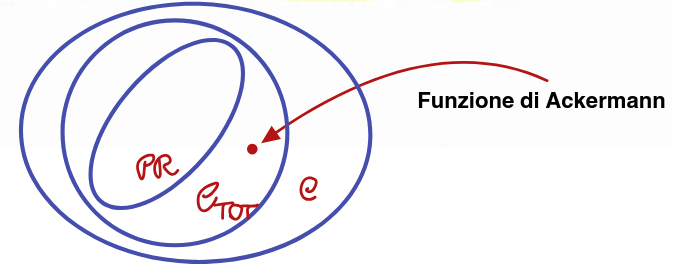
\includegraphics[width=0.75\linewidth]{images/insiemi-ricorsive-calcolabili}
		\caption{Le funzioni $\mathcal{PR}$ non coprono tutte le funzioni calcolabili totali, e in particolare, nessuna funzione parziale \textbf{non totale} è primitiva ricorsiva.}
	\end{figure}
	\chapter{Alcuni predicati decidibili e funzioni calcolabili}
	
	\section{Funzioni definite per casi}
	
	Siano $f_1(\vec{x}), \dots, f_k(\vec{x})$ funzioni \textbf{calcolabili totali} e $M_1(\vec{x}), \dots ,M_k(\vec{x})$ sono predicati \textbf{decidibili} tali che, per ogni $\vec{x}$, \textbf{esattamente uno} tra $M_1(\vec{x}), \dots ,M_k(\vec{x})$ è vero. Allora, la funzione 
	
	$$
	g(\vec{x}) =
	\begin{cases}
		f_1(\vec{x}) & \text{se } M_1(\vec{x}) \text{ è vero} \\
		\quad \vdots & \qquad \vdots \\
		f_k(\vec{x}) & \text{se } M_k(\vec{x}) \text{ è vero}\\
	\end{cases}
	$$
	
	è calcolabile. 
	
	\paragraph{Dimostrazione}
	
	Basta osservare che, con $c_{M_i}(\vec{x})$ funzione caratteristica del predicato $M_i(\vec{x})$, la seguente funzione è calcolabile
	
	$$
	g(\vec{x}) = c_{M_1}(\vec{x})\cdot f_1(\vec{x}) + \dots + c_{M_k}(\vec{x})\cdot f_k(\vec{x})
	$$
	
	La calcolabilità della funzione $g(\vec x)$ è verificata in quanto:
	\begin{itemize}
		\item Ogni termine $c_{M_i}(\vec x) \cdot f_i(\vec x)$ è ottenuto dalla composizione di tre funzioni, ossia: la funzione caratteristica del predicato $c_{M_i}$ (calcolabile in quanto decidibile per ipotesi), la funzione $f_i(\vec x)$ (calcolabile per ipotesi) e la \textbf{funzione prodotto} (calcolabile).
		\item La \textbf{somma di funzioni} calcolabili è calcolabile, in quanto ottenibile per composizione.
	\end{itemize}
	
	\section{Algebra della decidibilità}
	Se $M(\vec{x})$ e $Q(\vec{x})$ sono predicati \textbf{decidibili}, allora anche i seguenti predicati sono decidibili
	
	\begin{itemize}
		\item $\lnot M(\vec{x})$: $C_{\lnot M}(\vec{x}) = 1 \dotdiv M(\vec{x})$
		\item $M(\vec{x}) \land Q(\vec{x})$: $M(\vec{x}) \cdot Q(\vec{x})$
		\item $M(\vec{x}) \lor Q(\vec{x})$: $\mathrm{sign}(M(\vec{x}) + Q(\vec{x}))$, oppure $\max(M(\vec{x}), Q(\vec{x}))$
	\end{itemize}
	
	
	
	\newpage
	
	\section{Sommatorie e produttorie limitate}
	Tramite ricorsione, possiamo definire le operazioni di sommatoria e produttoria limitate, ossia:
	
	$$
	\sum_{z < y}f(\vec{x},z), \qquad \prod_{z < y}f(\vec{x},z)
	$$
	
	se $f(\vec{x},z)$ è calcolabile, anche le rispettive sommatorie e produttorie limitate sono calcolabili.
	
	\paragraph{Dimostrazione}
	Basta osservare che le sommatorie e le produttorie limitate soddisfano queste ricorsioni primitive:
	$$
	\begin{cases}
		\ \, \displaystyle\sum_{z<0}	f(\vec{x},z) = 0\\
		\displaystyle\sum_{z<y+1}f(\vec{x},z) = \sum_{z<y}f(\vec{x},z) + f(\vec{x}, y)
	\end{cases}
	\qquad
	\begin{cases}
		\ \,\displaystyle\prod_{z<0}	f(\vec{x},z) = 1\\
		\displaystyle\prod_{z<y+1}f(\vec{x},z) = \prod_{z<y}f(\vec{x},z) \cdot f(\vec{x}, y)
	\end{cases}
	$$
	
	sono quindi calcolabili. Lo stesso vale anche per
	
	\subsection{Corollario}
	Quanto detto in precedenza rispetto alle sommatorie e alle produttorie limitate, vale anche quando $y$ viene sostituito con una funzione calcolabile $k(\vec{x}, \vec{w})$. 
	$$
	\sum_{z < k(\vec{x}, \vec{w})}f(\vec{x},z), \qquad \prod_{z < k(\vec{x}, \vec{w})}f(\vec{x},z)
	$$
	La dimostrazione è per composizione. Un caso particolare, è quello di
	
	$$
	\sum_{z \leq y}f(\vec{x},z) = \sum_{z < y + 1}f(\vec{x},z), \qquad \prod_{z \leq y}f(\vec{x},z) = \prod_{z < y + 1}f(\vec{x},z)
	$$
	
	\section{Minimalizzazione limitata}
	È una versione \textit{bounded} dell'operazione di minimalizzazione, di cui parleremo nei prossimi capitoli. Indicato con $\mu z < y (f(\vec{x}, z) = 0)$, indica il minor $z$ minore di $y$ tale $f(\vec{x},z) = 0$\footnote{La condizione potrebbe essere diversa, ma questo è uno dei casi più tipici.}. La funzione in questione deve essere una \textbf{funzione totale} e \textbf{calcolabile}. In generale, diremo che
	
	$$
	\mu z <y ( f(\vec{x},z) = 0 )
	=
	\begin{cases}
		\text{minimo } z < y \text{ tale che} f(\vec{x},z) = 0 &\text{se tale $z$ esiste.}\\
		y  &\text{altrimenti}
	\end{cases}
	$$
	
	\paragraph{Dimostrazione} Dobbiamo dimostrare che $\mu z <y ( f(\vec{x},z) = 0 )$ sia calcolabile e totale. Che sia totale è triviale. Andiamo a costruire l'operatore di minimalizzazione limitata usando altre operazioni che sono notoriamente calcolabili.
	
	$$
	\prod_{u <y} \mathrm{sign}\big(f(\vec{x},u)\big) =
	\begin{cases}
		1 & \text{se } f(\vec{x},u) \neq 0 \text{ per ogni } u <y \\
		0 & \text{altrimenti}
	\end{cases}
	$$
	
	$$
	\sum_{z <y}\;\prod_{u <z} \mathrm{sign}\big(f(\vec{x},u)\big) =
	\begin{cases}
		y & \text{se } f(\vec{x},u)\neq 0 \text{ per ogni } u <y \\
		z_0 & \text{altrimenti, dove } z_0 \text{ è il minimo } z<y \text{ tale che } f(\vec{x},z)=0
	\end{cases}
	$$
	\begin{figure}[tbph]
		\centering
		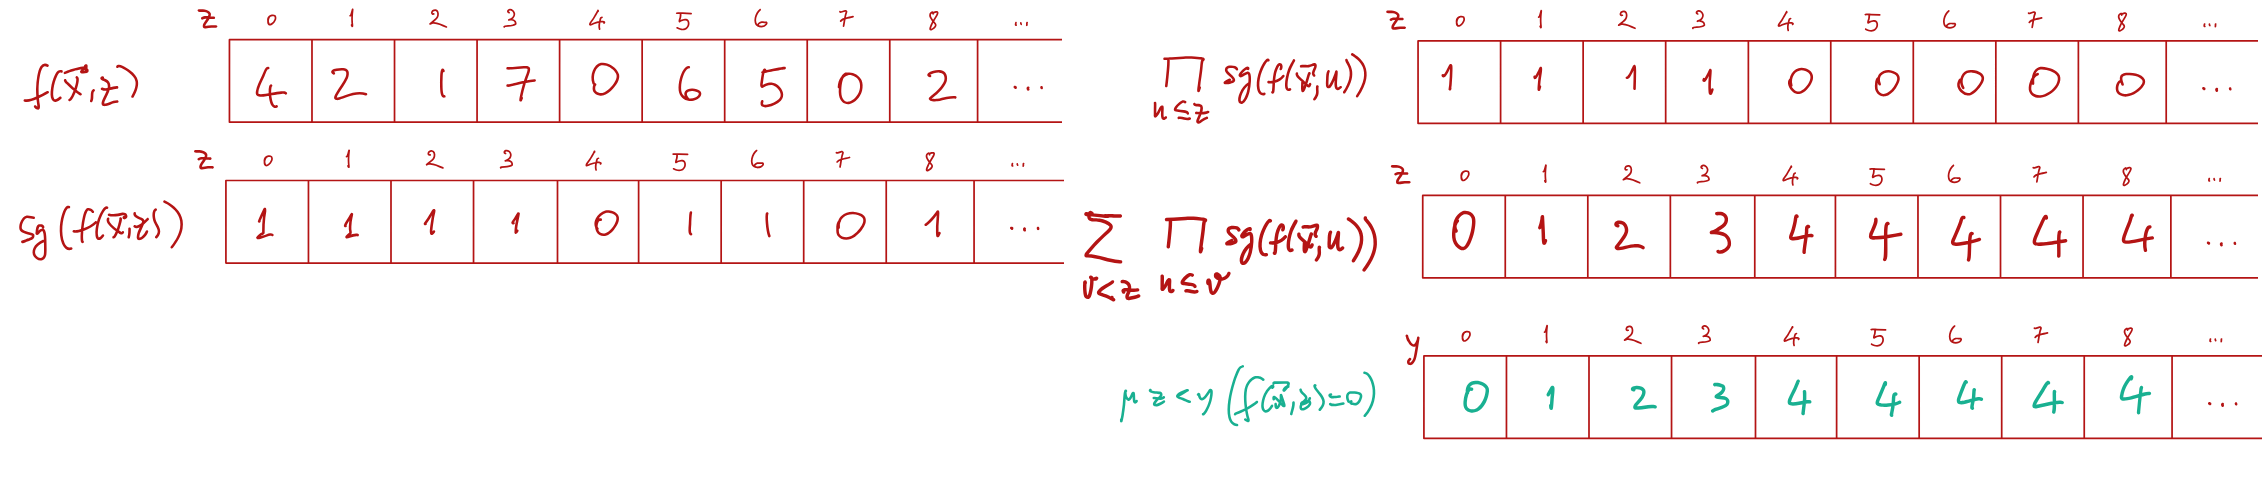
\includegraphics[width=1\linewidth]{images/boundedminimalization}
	\end{figure}
	
	$\sum_{z <y}\;\prod_{u <z} \mathrm{sign}\big(f(\vec{x},u)\big)$ è l'operatore di minimalizzazione limitata.
	
	
	\subsection{Corollario - minimalizzazione limitata da una funzione}
	Se $f(\vec{x},z)$ e $k(\vec{x}, \vec{w})$ sono calcolabili, $\mu z < k(\vec{x}, \vec{w}) (f(\vec{x},z) = 0)$ è calcolabile.
	
	\subsection{Corollario - minimalizzazione di predicati decidibili}
	Se $M(\vec{x},y)$ è calcolabile, $\mu z < y M(\vec{x},y)$ è calcolabile, e coincide col minimo valore di $z$ per cui il predicato è vero.
	
	$$
	\mu z < y\; M(\vec{x},y)
	=
	\mu z < y \big( C_M(\vec{x},z) = 1 \big)
	=
	\mu z < y \big( \overline{\mathrm{sg}}(C_M(\vec{x},z)) = 0 \big).
	$$
	
	
	\section{Quantificatori limitati}
	Sia $R(\vec{x}, y)$ un predicato decidibile. Allora, i seguenti predicati sono decidibili:
	
	$$
	(\forall z < y)R(\vec{x}, z), \qquad 
	(\exists z < y)R(\vec{x}, z)
	$$
	
	\paragraph{Dimostrazione: per ogni}
	Il predicato coincide con una produttoria limitata delle funzioni caratteristiche del predicato. È quindi calcolabile. 
	
	\paragraph{Dimostrazione: esiste un}
	Il predicato coincide col segno di una sommatoria limitata delle funzioni caratteristiche del predicato. È quindi calcolabile.
	
	\section{Codifiche per tuple}
	In generale, sappiamo che è possibile codificare in maniera effettiva sequenze di numeri in un singolo numero (in maniera totalmente univoca).
	Questo vuol dire che funzioni che operano su tuple, sono calcolabili. Questo apre le porte anche all'adattamento di funzioni ricorsive non primitive, in funzioni ricorsive primitive (vedremo un esempio sulla funzione di Fibonacci).
	
	
	\subsection{Codifiche per coppie di numeri}
	Dimostriamo che la codifica $\pi(x, y) = 2^x(2y+1) \dotdiv1$ è una biiezione calcolabile.
	
	\paragraph{Calcolabilità} È banale, nasce infatti da combinazione di funzioni calcolabili.
	
	\paragraph{Iniettività} 
	$$
	\begin{aligned}
	\pi(x,y) &= \pi(x',y')\\
	2^x(2y+1) \dotdiv 1&= 2^{x'}(2y'+1) \dotdiv 1\\
	2^x(2y+1) &= 2^{x'}(2y'+1) \\
	\end{aligned}
	$$
	
	DA FINIRE
	
	\subsection{Codifiche per sequenze di numeri}
	
	Vogliamo 
	
	Ogni numero $x \in \mathbb{N}$ può essere scritto nella forma
	$$
	x = \sum_{i=0}^{\ell} \alpha_i 2^i, \qquad \text{con } \alpha_i \in \{0,1\}
	$$
	univocamente.
	
	Quindi ogni $x>0$ ammette espressioni univoche della forma:
	$$
	x = 2^{b_1} + 2^{b_2} + \cdots + 2^{b_\ell}, \qquad 0 \le b_1 < b_2 < \cdots < b_\ell,\ \ell \ge 1
	$$
	
	$$
	x = 2^{a_1} + 2^{a_1+a_2+1} + \cdots + 2^{a_1+\cdots+a_\ell+(\ell-1)}, \qquad a_i \ge 0,\ \ell \ge 1
	$$
	
	Risultano quindi definite le seguenti funzioni:
	$$
	\alpha(i,x) = \alpha_i \qquad \text{(con } x = \sum_{i=0}^{\ell} \alpha_i 2^i\text{)}
	$$
	
	$$
	\ell(x) =
	\begin{cases}
		\ell & \text{se } x>0 \\
		0 & \text{altrimenti}
	\end{cases}
	$$
	
	$$
	b(i,x) =
	\begin{cases}
		b_i & \text{se } x>0 \text{ e } 1 \le i \le \ell(x) \\
		0 & \text{altrimenti}
	\end{cases}
	$$
	
	$$
	a(i,x) =
	\begin{cases}
		a_i & \text{se } x>0 \text{ e } 1 \le i \le \ell(x) \\
		0 & \text{altrimenti}
	\end{cases}
	$$
	
	
	
	\chapter{Minimalizzazione}
	Noto anche come \textbf{operatore di ricerca}.
	
	\section{Operazione di minimalizzazione}
	Mediante programmi URM è possibile effettuare la ricerca del più piccolo indice tale che si verifica una certa condizione. Non trovare l'indice porta a non terminazione.
	La \textbf{minimalizzazione} (non limitata) permette di definire una funzione $g(\vec{x})$ a partire da una funzione $f(\vec{x}, y)$ ponendo 
	
	$$
	g(\vec{x}) =_{def} \text{minimo $y$ tale che } f(\vec{x},y) = 0
	$$
	
	che in pseudo-codice equivale a:
	
		\begin{algorithm}
		\caption{Minimalizzazione in pseudocodice}
		\begin{algorithmic}
			\State $y = 0$
			\While{$f(\vec{x}), y \neq 0$} 
				\State $y = y+1$
			\EndWhile
			
			\State \Return $y$
		\end{algorithmic}
	\end{algorithm}
	
	\paragraph{Definizione} 
	Data una funzione $f(\vec{x},y)$ (anche parziale), poniamo
	
	$$
	\mu y ( f(\vec{x},y) = 0 )
	=
	\begin{cases}
		\text{minimo } y \text{ tale che} \\[4pt]
		\quad \cdot f(\vec{x},z)\downarrow \ \text{per ogni } z < y \\[4pt]
		\quad \cdot f(\vec{x},y) = 0, 
		\quad \text{se un siffatto } y \text{ esiste} \\[8pt]
		\uparrow \quad \text{altrimenti}
	\end{cases}
	$$
	
	dove $\mu$ è detto operatore di minimalizzazione. L'insieme $\mathcal C_{URM}$ è chiuso rispetto alla minimalizzazione.
	
	\subsection{Dimostrazione della calcolabilità}
	Vogliamo calcolare il seguente programma: $g(\vec{x}) = \mu y(f(\vec{x},z) = 0)$.
	
	\begin{algorithm}
		\caption{\textit{Minimalizzazione}}
		\begin{algorithmic}
			\State $T(1, m+1)$
			\State \qquad\vdots
			\State $T(n, m+n)$
			\State [$I_p$]:
			\State $R_1 \leftarrow f_F(R_{m+1}, \dots, R_{m+n}, R_{m+n+1})$
			\State $J(1, m+n+2, q)$
			\State $S(m+n+1)$
			\State $J(1,1,p)$
			\State $[I_q]: \ T(m+n+1, 1)$
		\end{algorithmic}
	\end{algorithm}
	
	
	\subsection{Corollario sulla minimalizzazione dei predicati decidibili}
	Il minimo valore $y$ tale che il predicato $R(\vec{x}, y)$ è vero, è calcolabile, in quanto
	
	$$
	\mu y (\overline{\mathrm{sign}}(C_R(\vec{x}, y) ) = 0)
	$$
	
	è calcolabile.
	
	\subsection{Funzioni parziali da funzioni totali}
	L'operatore di minimalizzazione, a causa della sua definizione, può derivare funzioni non totali a partire da funzioni totali! 
	
	\paragraph{Esempio} Se infatti la funzione $f(x,y) = |x - y^2|$ risulta essere calcolabile e totale, la funzione $g(x,y) \simeq \mu y(f(x,y) = 0)$ è calcolabile, ma non totale! Quando $x$ non è un quadrato perfetto, $\nexists y : y^2 = x \Rightarrow \nexists y = \sqrt{x}$. Quindi, la funzione calcolata a partire dalla $f$ totale e calcolabile, è
	
	$$
	g(x,y) = \begin{cases}
	\sqrt{x} & \text{se $x$ è un quadrato perfetto}\\
	\uparrow & \text{altrimenti}
	\end{cases}
	$$ 
	
	\section{Funzioni ricorsive parziali}
	
	La famiglia delle \textbf{funzioni ricorsive parziali} è quella delle funzioni generate per
	
	\begin{itemize}
		\item Composizione
		\item Ricorsione primitiva
		\item Minimalizzazione non limitata
	\end{itemize}
	
	di \textbf{funzioni iniziali}. Scopriremo che questa famiglia coincide con la famiglia delle funzioni \textbf{URM-calcolabili}.
	

	
	
	\chapter{Completezza delle funzioni ricorsive parziali}
	
	Faremo vedere che la famiglia di funzioni ricorsive parziali, è uguale alla funzioni URM-calcolabili.
	
	\section{Funzioni ricorsive parziali}
	La famiglia delle funzioni ricorsive parziali è quella delle funzioni definibili a partire dalle funzioni iniziali e con
	\begin{itemize}
		\item Composizione
		\item Ricorsione primitiva
		\item Minimalizzazione (non limitata)
	\end{itemize}
	
	Il nostro obiettivo sarà dimostrare che famiglia di funzioni ricorsive parziali, è uguale alla funzioni URM-calcolabili. Con la tesi di Church, vedremo come parleremo di funzioni calcolabili, e non solo URM-calcolabili.
	
	\section{Funzione di Ackermann}
	La funzione di Ackermann permette di esplicitare il limite delle funzioni ricorsive primitive. Il motivo per cui non può essere espressa tramite ricorsione primitiva, è la doppia ricorsione. Anche la funzione dei numeri di Fibonacci può essere ricondotta ad una forma primitiva ricorsiva, ma questa funzione no.
	
	$$
	\psi(x,y)=
	\begin{cases}
		\psi (0, y) = \begin{cases}
			1 & \text{se } y=0 \\
			2 & \text{se } y=1 \\
			y+2 & \text{se } y>1
		\end{cases}
		& \text{se } x=0 \\[14pt]
		\psi (x, 0) = 1 & \text{se } x\geq 1,\; y=0 \\[6pt]
		\psi(x+1,y+1) = \psi(x,\psi(x + 1,y)) 
		& \text{se } x\geq 1,\; y\geq 1
	\end{cases}
	$$
	
	per facilitare, cambiamo notazione. $\psi_x(y) \equiv \psi(x,y)$.
	
	$$
	\psi_x(y)=
	\begin{cases}
		\psi_0 (y) = \begin{cases}
			1 & \text{se } y=0 \\
			2 & \text{se } y=1 \\
			y+2 & \text{se } y>1
		\end{cases}
		& \text{se } x=0 \\[14pt]
		\psi_x (0) = 1 & \text{se } x\geq 1,\; y=0 \\[6pt]
		\psi_{x+1}(y+1) = \psi_x(\psi_{x+1}(y)) 
		& \text{se } x\geq 1,\; y\geq 1
	\end{cases}
	$$
	
	osserviamo che $\psi_{x+1}(y+1) = \psi_x(\psi_{x+1}(y)) = \psi_x^{(y+1)}(1)$. In generale dimostrare la calcolabilità di questa funzione non è facile.
	\subsection{Dimostrazione calcolabilità di $\lambda y.\psi_x(y)$}
	Faremo vedere per induzione su $x$ che la restrizione (unaria) $\lambda y.\psi_x(y)$ è calcolabile e totale. Osserviamo che non stiamo andando a valutare la funzione al variare di $x$, ma stiamo valutando su valori fissati di $x$.
	
	\begin{itemize}
		\item Caso base: $\lambda y.\psi_0(y)$. Questo termine è già presente nella definizione per casi.
		
		$$
		\psi_0(y) = \begin{cases}
			1 & \text{se } y=0 \\
			2 & \text{se } y=1 \\
			y+2 & \text{se } y>1
		\end{cases}
		$$
		\item Passo induttivo: l'ipotesi induttiva è che $\psi_x(y)$ sia calcolabile e totale. Si osservi quindi che la funzione $\psi_{x+1}$ può essere definita sulla seguente ricorsione primitiva (su $y$), in termini di $\psi_x$:
		
		$$
		\begin{cases}
		\psi_{x+1}(0) = 1\\
		\psi_{x+1} (y+1) = \psi_x(\psi_{x+1}(y))
		\end{cases}
		$$
	\end{itemize}
	
	pertanto, per induzione, $\psi_{x+1}$ è calcolabile e totale. Il fatto che questa funzione sia calcolabile per $x$ fissati, non significa che la funzione di Ackermann sia calcolabile.
	
	\begin{figure}[tbph]
		\centering
		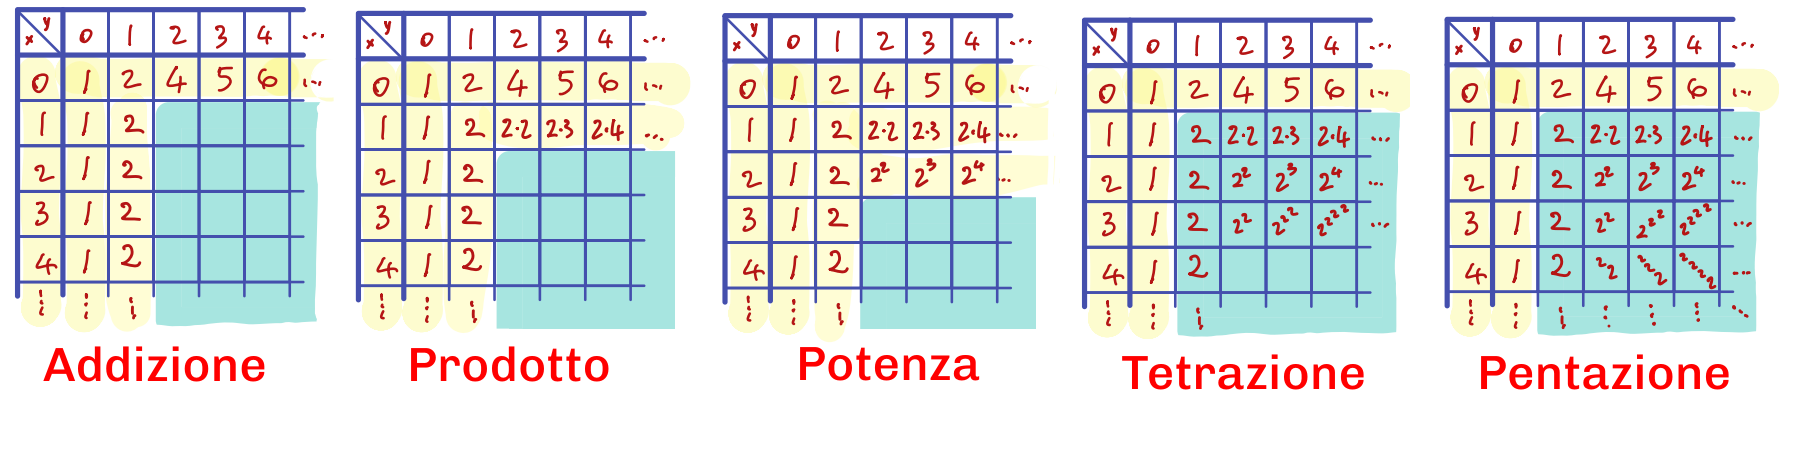
\includegraphics[width=1\linewidth]{images/ackermann}
	\end{figure}
	
	
	\subsection{Calcolabilità della funzione di Ackermann}
	Questa è la parte più difficile della dimostrazione.
	
	
	\paragraph{Triple} Intendiamo caratterizzare insiemi finiti $S$ di triple $(x,y,z) \in\mathbb{N}$ tali che, $\forall (x,y,z)\in \S$:
	\begin{itemize}
		\item $z=\psi(x,y)$
		\item $S$ contiene \textbf{tutte} le triple $(\overline{x},\overline{y}, \psi(\overline{x},\overline{x}))$ necessarie al calcolo di $\psi(x,y)$.
	\end{itemize}
	
	questi insiemi devono inoltre essere \textbf{validi}.
	
	\paragraph{Insiemi validi} Un insieme di triple $S$ è detto valido se le seguenti condizioni sono soddisfatte:
	\begin{itemize}
		\item se $(0,y,z) \in S$, allora $z = \begin{cases}
			1 & \text{se } y=0 \\
			2 & \text{se } y=1 \\
			y+2 & \text{se } y>1
		\end{cases}$.
		\item se $(x,0,z) \in S$, allora $z = 1$.
		\item se $(x+1,y+1,z) \in S$, allora $\exists u \in \mathbb{N}: \ (x+1, y, u), (x, u, z)$.
		
	\end{itemize}
	
	Osserviamo che $
	\psi(x+1,y+1)=
	\psi\big(\overbrace{x,\underbrace{\psi(x+1,y)}_{w}}^{z}\big)
	$. Un insieme finito di triple $S$ è detto \textbf{valido rispetto alla coppia} $(x,y) \in \mathbb{N}^2$ se
	\begin{itemize}
		\item $S$ è valido.
		\item $\exists u \in \mathbb{N} : (x,y,u) \in S$.
	\end{itemize}
	
	Possiamo poi definire un buon ordinamento $<_{\mathrm{lex}} \text{ su } \mathbb{N}\times\mathbb{N}$.
	$$
	(x,y) <_{\mathrm{lex}} (x',y')
	\;\Longleftrightarrow\;
	\big(x < x'\big) \;\vee\; \big(x = x' \land y < y'\big).
	$$
	
	\paragraph{Fatto 1} Se $S$ è valido, allora $\forall (x,y,z) \in S \Rightarrow z = \psi(x,y)$. Si dimostra per assurdo.
	
	{\huge TODO}
	
	\paragraph{Fatto 2} $\forall (x,y) \in \mathbb{N}^2, \exists S$ finito valido per $(x,y)$. Si dimostra per assurdo.
	
	{\huge TODO}
	
	\paragraph{Passo finale della dimostrazione}
	Una tripla $(x,y,z)$ può essere codificata in un singolo numero positivo $u = 2^x3^y5^z$, mentre un insieme finito di numeri positivi, e quindi di triple, può essere codificato in un singolo numero $v = p_{u_1}p_{u_2}\dots p_{u_k}$. Il set di triple codificato da $v$ è indicato con $S_v$.
	 
	Quindi, $(x,y,z) \in S_v \Leftrightarrow p_{2^x3^y5^z} \text{ divide }v$. Essendo questa una mutua implicazione, la decidibilità di un predicato implica la decidibilità dell'altro. Definiamo quindi la funzione
	
	$$
	R(x,y,v) \equiv \text{ "$v$ codifica un insieme valido di triple e $\exists z < v ((x,y,z) \in S_v)$"}.
	$$
	
	Essendo questo un predicato decidibile, è calcolabile anche la funzione
	
	$$
	f(x,y) = \mu v R(x,y,v)
	$$
	
	Ne consegue che la funzione di Ackermann è calcolabile tramite
	$$
	\psi(x,y) = \mu z ((x,y,z) \in S_{f(x,y)})
	$$
	
	\chapter{Loop Program}
	
	I loop program sono un sottoinsieme dei programmi URM.
	
	\section{Istruzioni dei loop program}
	L'istruzione di salto condizionato, viene sostituita con l'istruzione loop, che consiste in realtà in due keyword: $\mathrm{Loop}(n) , \mathrm{End}$. Somiglia un po' a un ciclo for, in quanto, sia $k$ il valore del registro $R_n$, il programma presente tra le keyword viene ripetuto $k$ volte.
	
	\subsection{Mappare Loop program in un programma URM}
	
	\begin{algorithm}
		\caption{\textit{Loop program}}
		\begin{algorithmic}
		\State \textbf{Loop}(n)
		\State \quad P
		\State \textbf{End}
		\end{algorithmic}
	\end{algorithm}
	
	
	\begin{algorithm}
		\caption{\textit{Loop program in URM}}
		\begin{algorithmic}
			\State T(n, m*)
			\State Z(m*+1)
			\State $[I_p]:$
			\State J(m* + 1, m*, q)
			\State P
			\State S(m*+1)
			\State J(1, 1, p)
		\end{algorithmic}
	\end{algorithm}
	
	\section{Gerarchia dei Loop program}
	Distinguiamo i loop program secondo il numero di cicli loop annidati. Usiamo quindi
	\begin{itemize}
		\item $L_0$: insieme dei loop program che presentano sole istruzioni $Z(n), S(n), T(m,n)$.
		\item $L_{k+1}$: insieme dei loop program costituiti da $Z(n), S(n), T(m,n)$ e $Loop$ contenenti $P \in L_k$.
	\end{itemize}
	
	È una notazione ricorsiva. Banalmente $L_k \subset L_{k+1}$ per $k \in \mathbb{N}$.
	
	\subsection{Gerarchia delle \textit{funzioni} calcolate dai Loop program}
	Per ogni $n \geq 0$, indichiamo con $\mathcal L_n$ l'insieme delle funzioni \textbf{calcolate da programmi} in $L_n$.   
	
	\paragraph{Funzione di Ackermann \textit{n}-esima}
	Osserviamo che, data $\psi_{n+1}$ funzione di Ackermann ennesima $\psi_{n+1} \in \mathcal{L}_{n+1} \backslash \mathcal{L}_{n}$.
	
	\section{Funzioni primitive ricorsive e i Loop Program}
	Indichiamo con $\mathcal L = \bigcup_{n=0}^\infty \mathcal{L}_n$, ossia l'insieme di tutti i loop program.
	Vogliamo dimostrare che
	$$
	\mathcal{PR} = \bigcup_{n=0}^\infty \mathcal{L}_n = \mathcal{L}
	$$
	
	La dimostrazione consisterà in
	\begin{enumerate}
		\item Dimostrare che le funzioni iniziali appartengono a $\mathcal L_0$.
		
		\item Dimostrare che $\bigcup_{n=0}^\infty \mathcal{L}_n$ è chiuso rispetto a composizione e ricorsione primitiva, concludendo che $\mathcal{PR} \subseteq \bigcup_{n=0}^\infty \mathcal{L}_n$.
		
		\item Dimostrare $\mathcal{PR} \supseteq \bigcup_{n=0}^\infty \mathcal{L}_n$ per induzione su $n$.
	\end{enumerate}
	
	\paragraph{1. Dimostrazione funzioni iniziali}
	Le funzioni iniziali sono in $\mathcal L_0$, e coincidono con le uniche istruzioni ammesse da $\mathcal L_0$. Triviale.
	
	\paragraph{2.1. Dimostrazione composizione} Siano $f(y_1, \dots, y_k), g_1(\vec{x}), \dots, g_k(\vec{x}) \in \mathcal L_p$. Sia $h(\vec{x}) = f(g_1(\vec{x}), \dots g_k(\vec{x}))$. Il programma che calcola la composizione $h(\vec{x})$ è il già ben noto
	\begin{algorithmic}
		\State $T(1, m+1)$
		\State $\quad \vdots$ 
		\State $T(n,m+n)$
		\State $R_{m+n+1} \gets f_{G_1}(R_{m+1}, \dots, R_{m+n})$
		\State $\quad \vdots$
		\State $R_{m+n+k} \gets f_{G_k}(R_{m+1}, \dots, R_{m+n})$
		\State $R_1 \gets f_{F}(R_{m+n+1}, \dots, R_{m+n+k})$
	\end{algorithmic}
	e si trova in $\in L_p$.
	
	\paragraph{2.2. Dimostrazione ricorsione primitiva} Lo stesso vale per la ricorsione primitiva. Infatti, se le funzioni delle equazioni ricorsive $f(\vec{x}), g(\vec{x}, y, z) \in \mathcal L_p$, allora la funzione $h(\vec{x}, y)$ definita per ricorsione primitiva si troverà in $\mathcal L_{p+1}$.
	
	Di conseguenza, siano $F$ e $G$ che calcolano le funzioni $f, g$, allora $F, G \in L_p$, mentre il programma che calcola $h(\vec{x}, y)$ è in $L_{p+1}$, in quanto ottenuto da un loop che itera per $y$ volte, ovviamente calcolabile.
	
	Abbiamo pertanto dimostrato che $\bigcup_{n=0}^\infty \mathcal{L}_n$ è chiuso rispetto a composizione e ricorsione primitiva.
	
	\paragraph{3.0.1. Notazione vettoriale} Prima di dimostrare l'ultima inclusione della dimostrazione, introduciamo la seguente notazione:
	la seguente funzione 
	$$
	\vec{f}: \mathbb{N}^m \to \mathbb{N}^n
	$$
	
	è una funzione vettoriale che prende in input elementi di tipo $\vec{x} \in \mathbb{N}^m$, e cui output è dato da $\vec{f}(\vec{x}) = (f_1(\vec{x}), \dots, f_n(\vec{x}))$. Ciascuna delle componenti di $f$, ossia $f_i \ \forall i \in \{1,\dots, n \}$, è del tipo $f_i: \mathbb{N}^m \to \mathbb{N}$.
	È detta anche funzione vettoriale di tipo $(m,n)$.
	Una funzione vettoriale di tipo $(m,n)$ si dice \textbf{calcolabile} se ciascuna delle sue componenti $f_i$ è calcolabile.
	
	\paragraph{3.0.2. Proprietà delle funzioni vettoriali}
	\begin{itemize}
		\item Composizione: se due funzioni vettoriali $\vec{f}, \vec{g}$ rispettivamente di tipo $(m,n)$ ed $(n,p)$ sono primitive ricorsive, tale lo è la loro composizione $\vec{f} \circ \vec{g}$, che sarà di tipo $(m,p)$.
	\end{itemize}
	
	\chapter{Altri approcci alla computabilità e tesi di Church}
	
	\section{Altri approcci alla computabilità}
	
	Il modello URM è uno dei modelli più recenti usati nello studio della calcolabilità. Tra gli approcci alla calcolabilità, questi sono alcuni dei modelli più noti:
	\begin{itemize}
		\item Godel - Herbrand - Kleene: funzioni ricorsive generali.
		\item Church: $\lambda$-calcolo.
		\item Godel - Kleene: funzioni $\mu$-ricorsive e funzioni ricorsive parziali. $\star$
		\item Turing: funzioni calcolabili mediante macchine di Turing. $\star$
		\item Post: funzioni definite mediante sistemi deduttivi canonici.
		\item Sheperdson-Sturgis: funzioni URM-calcolabili. $\star$
	\end{itemize}
	
	i modelli $\star$ saranno oggetti del nostro studio.
	
	\paragraph{Risultato della teoria della calcolabilità} Tutti i modelli precedentemente proposti caratterizzano la medesima classe di \textbf{funzioni calcolabili}, che abbiamo precedentemente denotato con $\mathcal{C}$, per cui non ha più senso dire $\mathcal{C}_\text{URM}$.
	
	\section{Funzioni ricorsive parziali (Godel - Kleene)}
	La classe $\mathcal{R}$ delle \textbf{funzioni ricorsive parziali} è la più piccola delle famiglie di funzioni parziali che
	\begin{itemize}
		\item Contiene le funzioni iniziali $\underline 0, x+1, \bigcup_{i}^n$.
		\item È chiusa rispetto a \textbf{composizione}, \textbf{ricorsione primitiva}, \textbf{minimalizzazione}.
	\end{itemize}
	
	Godel e Kleene hanno inizialmente portato la loro attenzione sulla classe $\mathcal{R}_0$, ossia delle \textbf{funzioni $\mu$-ricorsive}, che coincide con $\mathcal{R}$ e ammette la minimalizzazione \textbf{solo se non consente funzioni parziali}.
	
	$$
	\mathcal{R}_0 = \mathcal{R} \cap TOT
	$$
	
	\subsection{Tutte le funzioni ricorsive parziali sono calcolabili}
	$$
	\mathcal{R} = \mathcal{C}_{URM}
	$$
	
	\paragraph{Dimostrazione} 
	
	Per quanto visto in precedenza, $\mathcal{R} \subseteq \mathcal{C}_{URM}$.

	Viceversa, sia $f(\vec{x})$ una funzione URM-calcolabile da un programma $P = I_1, I_2, \dots, I_s$. Senza perdere di generalità, possiamo supporre $P$ sia in forma standard, e che non ci siano istruzioni di salto che facciano passare all'istruzione subito successiva. Definiamo quindi un \textit{passo} come l'esecuzione di un'istruzione. 
	
	Consideriamo adesso le seguenti le seguenti funzioni relative alla computazione di $P$.
	
	$$
	c(\vec{x}, t) = \begin{cases}
	R_1 &\text{dopo $t$ passi della computazione $P(\vec{x})$ se questa non si è interrotta.}\\
	R_1 &\text{a fine computazione, se si è interrotta.}
	\end{cases}
	$$
	
	$$
	j(\vec{x}, t) =  \begin{cases}
		\text{numero della prossima istruzione} &\text{dopo $t$ passi di $P(\vec{x})$ se questa non si è interrotta.}\\
		0 &\text{se si è interrotta.}
	\end{cases}
	$$
	
	queste sono evidentemente funzioni totali. Osserviamo quindi che
	
	$$
	f_P^{(n)}(\vec{x})\downarrow \Leftrightarrow \mu t (j(\vec))
	$$
NON STO CAPENDO NULLA
	
	\section{Macchine di Turing}
	Una macchina di Turing $M$è un dispositivo finito che effettua operazioni primitive su un nastro infinito. Il nastro infinito è suddiviso in caselle che possono contenere un simbolo tratto da una lista finita di simboli, detto \textbf{alfabeto della macchina}. $s_0$ è il simbolo \textit{"blank"}, o $B$.
	
	$M$ può effettuare operazioni di lettura e scrittura (tramite una testina), e spostarsi a sinistra o a destra sul nastro. Ha inoltre un'unità di controllo costituita da un insieme finito di quadruple.
	
	\paragraph{Quadruple} Ciascuna di queste quadruple è nella forma
	
	$$
	q_i \ s_j \ \alpha \ q_l
	$$
	
	con $q_i$ stato della macchina, $s_j$ carattere letto, $\alpha \in \{L, R, s_0, \dots, s_k\}$ e $q_l$ nuovo stato. Ogni quadrupla definisce quindi quale azione effettuare (spostamento a sx, a dx o sovrascrittura di quale simbolo), quando la macchina legge un carattere in un determinato stato, e in quale stato transitare.
	
	\paragraph{Convezione sul contare} Negli usi che faremo, rappresenteremo il numero $n$ con $n$ caselle contenenti il simbolo $1$. La funzione che conta il numero di occorrenze di $1$ sul nastro è Turing-calcolabile.
	
	\subsection{Funzioni Turing calcolabili}
	Una funzione parziale si dice \textbf{Turing-calcolabile} se esiste una macchina di Turing che la calcola. La famiglia delle funzioni Turing-calcolabili si indica con $\mathcal{C}_{TUR}$.
	
	\subsection{Equivalenza tra URM e TM}
	Le funzioni ricorsive parziali $\mathcal R$ sono URM-calcolabili, ma anche Turing-calcolabili, ossia
	
	$$
	\mathcal{C}_{URM} = \mathcal{R}= \mathcal{C}_{TUR}
	$$
	
	e ciò è dimostrabile per \textbf{simulazione}.
	
	\newpage
	
	\section{Tesi di Church-Turing}
	La tesi di Church Turing è uno dei pilastri teorici dell'informatica moderna, e ha un ruolo fondamentale nella teoria della computabilità.
	Afferma che:
	\begin{center}
	\textit{La classe delle funzioni \textbf{intuitivamente} (umanamente) calcolabili coincide con la classe $\mathcal{C}_{URM}$, ossia quella delle funzioni URM-calcolabili. Lo stesso vale per le macchine di Turing, e qualsiasi altro sistema formale di computazione. È calcolabile tutto ciò che può essere calcolato da una macchina di Turing.}
	\end{center}
	
	A supporto di questa tesi, abbiamo che:
	\begin{itemize}
		\item La tesi di Church-Turing risulta essere il teorema fondamentale della calcolabilità, in quanto tutti i sistemi di calcolabilità sembrano convergere alla stessa classe di funzioni calcolabili.
		\item Si ha una collezione di funzioni per la quale esiste una dimostrazione di appartenenza a $\mathcal{C}_URM = \mathcal{C}_TUR = \mathcal{R}$.
		\item La possibilità di simulare effettivamente programmi URM.
		\item La mancanza di controesempi di funzioni effettivamente\footnote{Nella teoria della calcolabilità, un algoritmo effettivo (o procedura effettiva) è un insieme finito di istruzioni precise, non ambigue e meccaniche che, se applicato a un problema, produce una soluzione corretta in un numero finito di passi. Deve essere eseguibile da un essere umano o macchina senza intuizione, garantendo lo stesso risultato.} calcolabili ma non URM-calcolabili.
	\end{itemize}
	
	\subsection{La potenza della tesi di Church-Turing}
	Basandosi sulle prove precedentemente descritte, tutti i matematici hanno accettato la tesi di Church, la quale risulta essere uno strumento estremamente potente nelle dimostrazioni. Piuttosto che usare un modello teorico, come quello URM, o le macchine di Turing, possiamo procedere nel seguente modo.
	
	\paragraph{Dimostrazione della calcolabilità \textit{per tesi di Church}} Desideriamo dimostrare la calcolabilità della funzione $f$. Definiamo (in linguaggio naturale, tramite diagrammi o schemi) un algoritmo, e forniamo una dimostrazione informale ma rigorosa relativa al fatto che l'algoritmo calcola effettivamente la funzione $f$. Appelliamoci poi alla tesi di Church e concludiamo immediatamente dicendo che $f$ è URM-calcolabile. 
	
	\subsubsection{Estratto dal libro (che personalmente adoro) riguardo la tesi di Church-Turing}

	\begin{verbatim}
	Note that in using Church’s thesis we are not proposing to abandon all
	thought of proof, as if Church’s thesis is a magic wand which we can wave instead. 
	A proof by Church’s thesis will always involve proof that is
	careful, and sometimes complicated, although informal. [...]
	Church’s thesis not only keeps proofs shorter, but also prevents the
	main idea of a proof or construction from being obscured by a mass of
	technical details. It remains, however, an expression of faith or
	confidence. The validity of faith depends on the evidence that can be
	mustered. In the case of Church’s thesis, there is the mathematical
	evidence already outlined. For the practised student there is the addi
	tional evidence of his own experience in translating informal algorithms
	into formal counterparts. For the beginner, our use of Church’s thesis in
	subsequent chapters may call on his willingness to place confidence in the
	ability of others until self confidence is developed.
	\end{verbatim}
	\chapter{Enumerazione delle funzioni calcolabili}
	
	\section{Enumerazione}
	Un insieme infinito $X$ è enumerabile se esiste una biezione $f: X \to N$. Se $f$ ed $f^{-1}$ sono anche \textbf{effettivamente calcolabili}, l'insieme $X$ si dirà \textbf{effettivamente enumerabili}.
	
	Nello specifico, \textbf{una enumerazione di un insieme} $X$ è una suriezione $g: \mathbb{N} \to X$, (indicata con $X = \{x_0,x_1,x_2, \dots\}$). Quando $g$ è iniettiva, diremo anche che è un'\textbf{enumerazione senza ripetizioni}. 
	
	\subsection{Alcuni risultati tecnici}
	
	I seguenti insieme sono effettivamente enumerabili:
	
	\begin{enumerate}
		\item $\mathbb{N}\times\mathbb{N}$
		\item $\mathbb{N}^+\times\mathbb{N}^+\times\mathbb{N}^+$
		\item $\bigcup_{k>0}\mathbb{N}^k$
	\end{enumerate}
	
	\section{Enumerabilità dei programmi}
	
	Dimostriamo passo passo l'enumerabilità dei programmi, partendo dalla consapevolezza che, un programma qualsiasi, è una sequenza finita di istruzioni. Dimostriamo che l'insieme delle istruzioni è enumerabile.
	
	\subsection{Enumerabilità delle istruzioni}
	Dimostriamo l'enumerabilità dell'insieme delle istruzioni, indicato con $g$, definendo una biezione $\beta: \mathcal g \to \mathbb{N}$.
	
	\section{Numero di Gödel}
	
	Dato un programma $P \in \mathcal P$, $\gamma(P)$ è detto \textbf{numero di   Gödel} di $P$ (o codice di $P$). Inoltre, poniamo $P_n = \gamma^{-1}(n)$.
	
	\subsection{Notazioni utili}
	\begin{itemize}
		\item $\varphi_a^{(n)}$: la funzione $n$-aria calcolata da $P_a$.
		\item $W_a^{(n)}$: il dominio di $\varphi_a^{(n)} = \{\}$
	\end{itemize}
	
	\section{Enumerabilità delle funzioni}
	$C_n = \{\varphi_a^{(n)}: a \in \mathbb{N}\}$, ossia l'insieme delle funzioni calcolabili, è enumerabile.
	
	\section{Diagonalizzazione di Cantor}
	
	Data un'enumerazione $x_0, x_1, x2$ di funzioni parziali da $\mathbb{N}$ in $\mathbb{N}$, il \textbf{metodo diagonale di Cantor} consente di costruire una funzione $x$ da $\mathbb{N}$ in $\mathbb{N}$, diversa da tutte le funzioni $x_i$ dell'enumerazione 
	
	$$
	\begin{array}{c|ccccc}
		& 0 & 1 & 2 & 3 & \cdots \\ \hline
		\chi_0 & \chi_0(0) & \chi_0(1) & \chi_0(2) & \chi_0(3) & \cdots \\
		\chi_1 & \chi_1(0) & \chi_1(1) & \chi_1(2) & \chi_1(3) & \cdots \\
		\chi_2 & \chi_2(0) & \chi_2(1) & \chi_2(2) & \chi_2(3) & \cdots \\
		\vdots & \vdots & \vdots & \vdots & \vdots & \ddots
	\end{array}
	$$
	
	\subsection{Teorema sull'esistenza di una funzione totale, unitaria e non calcolabile}
	
	Esiste una funzione totale, unitaria e non calcolabile.
	
	$$
	f(n)=
	\begin{cases}
	\varphi_n(n) +1 &\text{se } \varphi_n(n)\downarrow\\
	0 &\text{se } \varphi_n(n)\uparrow
	\end{cases}
	$$
	
	\chapter{Decidibilità}
	
	\section{Teorema \textit{s-m-n }o di parametrizzazione}
	
	Sia $f(x,y)$ una funzione calcolabile, e dato $a \in \mathbb{N}$, poniamo 
	
	$$
	f_a(y) =_{def} f(a,y)
	$$
	
	$f_a$ è calcolabile, quindi $f_a = \varphi_{e_a}$
	
	
	
	\chapter{Programmi universali}
	
	\section{Programma universale}
	Si consideri la funzione $\psi(x,y) =_{def} \varphi_x(y)$. Questa funzione è universale, in quanto, ponendo $g_m(y) =_def \psi(m,y)$, la sequenza di $g_0, g_1, g_2, \dots$ contiene tutte le funzioni unarie calcolabili $\varphi_0^{(1)}, \varphi_1^{(1)}, \varphi_2^{(1)}, \dots$.
	
	\subsection{Calcolabilità della funzione universale}
	Per ogni arietà $n \geq 1$, la funzione universale $\psi_U^{(n)}$ è calcolabile.
	
	\paragraph{Dimostrazione}
	
	
	\section{Esistenza di funzione \textit{totale} calcolabile non primitiva ricorsiva}
	Esiste una funzione \textit{totale} calcolabile non primitiva ricorsiva
	\paragraph{Dimostrazione}
	
	
	
	
	\section{Operazioni effettiva su funzioni calcolabili}
	Ci chiediamo se sia possibile manipolare in maniera effettiva funzioni o insiemi infiniti (ricorsivamente enumerabili\footnote{Gli insiemi ricorsivamente enumerabili sono collezioni di elementi (solitamente numeri naturali) per i quali esiste un algoritmo capace di elencarne i membri o di riconoscere quelli validi in tempo finito}): in alcuni casi, questo è possibile, tramite applicazione del teorema di parametrizzazione!
	
	\subsection{Esempio 1}
	Date $\varphi_x, \varphi_y$, calcolare un indice di $\varphi_x\varphi_y$.
	
	$$
	\begin{aligned}
		\varphi_x(z)\cdot \varphi_y(z)
		&=
		\psi_U(y_1,z)\cdot \psi_U(y,z) \\
		&= \varphi^{(3)}_e(x,y,z) \\
		&= \varphi_{S_1^2(e,x,y)}(z) \\
		&= \varphi_{k(x,y)}(z)
		\quad
		\big(\text{con } k(x,y):=S_1^2(e,x,y)\ \text{totale calcolabile}\big) \\
		&\Longrightarrow\quad
		\varphi_x\cdot \varphi_y = \varphi_{k(x,y)}
	\end{aligned}
	$$
	
		\subsection{Esempio 2}
		Esiste una funzione calcolabile totale $g(x)$ tale che $(\varphi_x)^2 = \varphi_{g(x)}$.
	
	$$
	\begin{aligned}
		\varphi_x(z)\cdot \varphi_y(z)
		&=
		\psi_U(y_1,z)\cdot \psi_U(y,z) \\
		&= \varphi^{(3)}_e(x,y,z) \\
		&= \varphi_{S_1^2(e,x,y)}(z) \\
		&= \varphi_{k(x,y)}(z)
		\quad
		\big(\text{con } k(x,y):=S_1^2(e,x,y)\ \text{totale calcolabile}\big) \\
		&\Longrightarrow\quad
		\varphi_x\cdot \varphi_y = \varphi_{k(x,y)}
	\end{aligned}
	$$
	
	
	
	
	
	\chapter{???}
	
	\section{Problemi indecidibili della teoria della calcolabilità}
	
	\subsection{Halting problem}
	Il problema "$x \in W_x$" è indecidibile. Si dimostra verificando che la funzione 
	
	
	
	\chapter{Definizioni, sinonimi, chiarimenti}
	
	\section{Sinonimi}
	\begin{itemize}
		\item \textit{Calcolabilità} e \textit{computabilità}.
		\item \textit{Composizione} e \textit{sostituzione}.
	\end{itemize}
	
	
	
	
\end{document}